\documentclass[conference]{IEEEtran}
\usepackage{cite}
\usepackage{amsmath,amssymb,amsfonts}
\usepackage{algorithmic}
\usepackage{graphicx}
\usepackage{textcomp}
\usepackage{xcolor}
\def\BibTeX{{\rm B\kern-.05em{\sc i\kern-.025em b}\kern-.08em
    T\kern-.1667em\lower.7ex\hbox{E}\kern-.125emX}}

\begin{document}

\title{Digitalización de Historias Clínicas}

\author{
    \IEEEauthorblockN{Jerónimo Muñoz Gálvez}
    \IEEEauthorblockA{
        \textit{Escuela de Ciencias e Ingeniería} \\
        \textit{Universidad del Rosario} \\
        Bogotá, Colombia \\
        jeronimo.munoz@urosario.edu.co
    }
    \and
    \IEEEauthorblockN{María Isabela Borda Robles}
    \IEEEauthorblockA{
        \textit{Facultad de Economía} \\
        \textit{Universidad del Rosario} \\
        Bogotá, Colombia \\
        mariai.borda@urosario.edu.co
    }
    \and
    \IEEEauthorblockN{Samuel Alejandro Galindo Martinez}
    \IEEEauthorblockA{
        \textit{Escuela de Ciencias e Ingeniería} \\
        \textit{Universidad del Rosario} \\
        Bogotá, Colombia \\
        samuela.galindo@urosario.edu.co
    }
    \and
    \IEEEauthorblockN{Victoria Rios Rodriguez}
    \IEEEauthorblockA{
        \textit{Escuela de Ciencias e Ingeniería} \\
        \textit{Universidad del Rosario} \\
        Bogotá, Colombia \\
        victoria.rodriguez@urosario.edu.co
    }
}

\maketitle

\begin{abstract}
Este documento tiene como objetivo la condensación del proceso investigativo y productivo llevado a cabo por este grupo de proyecto para la digitalización, edición y manejo de historias medicas del consultorio de los Doctores Ivonne Robles y Henry Borda para la gestión de citas y tratamientos.
\end{abstract}

\section{Introducción}

La gestión de información en el sector salud representa un elemento fundamental para garantizar la calidad del servicio, el seguimiento adecuado de los pacientes y el cumplimiento de normativas legales. En consultorios privados, donde el flujo de pacientes puede ser constante, el manejo manual de historias clínicas puede generar retrasos y dificultades en la organización de la información.

El presente proyecto surge a partir de la necesidad identificada en el consultorio odontológico de los doctores Ivonne Robles y Henry Borda, quienes se especializan en ortodoncia, ortopedia maxilofacial, periodoncia e implantología. Actualmente, el manejo de historias clínicas se realiza de manera física, lo cual implica tiempos de búsqueda prolongados, dificultad en el seguimiento de tratamientos y limitaciones en el control de pagos y citas.

Con el fin de optimizar estos procesos, se propone el diseño e implementación de una base de datos que permita digitalizar las historias clínicas, organizar citas y registrar la evolución de los tratamientos, garantizando acceso rápido, seguridad de la información y cumplimiento de lineamientos establecidos por la Secretaría de Salud. 

\section{Planteamiento del Problema}

El consultorio odontológico está presentando dificultades en la organización y gestión de las historias clínicas debido a que estas se almacenan en un formato físico lo cual a menudo puede llevar al error humano, sumado a esto, el promedio estimado de atención diaria es de 8 a 12 pacientes lo cual incrementa el volumen de información, la cantidad de datos por almacenar y la probabilidad de errores administrativos.

En el proceso de análisis de la situación se pudieron encontrar los siguientes problemas:

\begin{itemize}
    \item Retrasos en la búsqueda de historias clínicas físicas.
    \item Falta de control claro sobre pagos realizados y citas pendientes.
    \item Dificultad para llevar un seguimiento continuo de tratamientos.
    \item Riesgo asociado a la pérdida de información confidencial.
\end{itemize}

Adicionalmente, las historias clínicas deben cumplir con lineamientos establecidos por la Secretaría de Salud de Bogotá, los cuales actualmente se diligencian manualmente en cada modificación o apertura de historia clínica.

En este contexto, surge la siguiente pregunta de investigación:

\textbf{¿Cómo puede una base de datos estructurada mejorar la gestión de historias clínicas, citas, pagos y seguimiento de tratamientos en un consultorio odontológico privado?}

\section{Justificación}

La implementación de una base de datos para la gestión de historias clínicas representa una solución tecnológica que permite mejorar la organización interna del consultorio, optimizar tiempos de atención y fortalecer la confianza del paciente.

La digitalización de la información facilitará el acceso rápido a antecedentes clínicos, diagnósticos y planes de tratamiento, reduciendo el tiempo de transición entre pacientes. Asimismo, permitirá llevar un control estructurado de citas programadas, pagos realizados y evoluciones clínicas.

Adicionalmente, el almacenamiento digital contribuye a la protección de datos sensibles y al cumplimiento de los requisitos normativos establecidos por las autoridades de salud. Por estas razones, el desarrollo de este sistema constituye una mejora significativa en la eficiencia operativa del consultorio.

\section{Objetivos}

\subsection{Objetivo General}

Diseñar una base de datos que permita digitalizar y gestionar las historias clínicas, citas y tratamientos en el consultorio odontológico privado.

\subsection{Objetivos Específicos}

\begin{itemize}
    \item Optimizar la búsqueda de historias clínicas mediante un sistema de consulta por nombre, número de documento o número telefónico.
    \item Integrar un módulo para el registro organizado de diagnósticos, pronósticos y planes de tratamiento.
    \item Implementar un sistema de seguimiento evolutivo para cada paciente.
    \item Permitir la carga de archivos complementarios como radiografías e imágenes diagnósticas.
    \item Clasificar pacientes según antecedentes sistémicos relevantes para mejorar la atención clínica.
\end{itemize}

\section{Alcance del Proyecto}

El proyecto contempla el diseño e implementación de una base de datos relacional orientada a la gestión interna del consultorio odontológico. El sistema permitirá digitalizar y organizar la información clínica y administrativa bajo los siguientes componentes funcionales:

\subsection{Delimitación Funcional}

\begin{itemize}
    \item Gestión de citas y pagos vinculados a cada paciente.
    \item Consulta rápida de historias clínicas mediante nombre, cédula o número de contacto.
    \item Registro médico para ingreso de diagnósticos, recetas y planes de tratamiento.
    \item Gestión de archivos en formato PDF como soporte clínico.
    \item Sistema básico de alertas visuales para advertencias médicas (ej. alergias).
    \item Control de acceso exclusivo para el personal interno del consultorio.
\end{itemize}

\subsection{Alcances Excluidos}

\begin{itemize}
    \item No se implementará despliegue en servicios en la nube como Google Cloud o Microsoft Azure.
    \item No habrá acceso remoto ni portal para pacientes.
    \item No se incluirá un sistema avanzado de cruce automático de medicamentos por componentes.
\end{itemize}

\section{Estructura del Sistema}

La base de datos estará organizada en los siguientes módulos principales las cuales se completaran con sus respectivas clases:

\begin{itemize}
    \item Gestión de usuarios (doctores y asistentes).
    \item Registro de pacientes.
    \item Gestión de citas.
    \item Historias clínicas completas.
    \item Control de pagos y evolución de tratamientos.
\end{itemize}

\section{Requisitos Funcionales}
Los siguientes requisitos funcionales son considerados críticos para el diseño y la implementación de la base de datos del sistema de historias clínicas odontológicas. Estos requisitos definen las entidades, atributos, relaciones y reglas de negocio fundamentales que la base de datos debe soportar.

\begin{enumerate}

    \item \textbf{Creación de Historias Clínicas (RQF019, RQF01)}: El sistema debe permitir la creación de un registro único e integral para cada paciente. Este registro, o historia clínica, actuará como la entidad principal del sistema, agrupando toda la información demográfica, clínica y administrativa del paciente.

    \item \textbf{Unicidad de Pacientes (RQF020)}: La base de datos debe garantizar la integridad y unicidad de los datos del paciente. Para ello, debe implementar mecanismos que prevengan la creación de registros duplicados, validando la información de identificación (como número de cédula o ID) antes de la inserción de un nuevo registro.

    \item \textbf{Gestión de Firmas Digitales (RQF025)}: La base de datos debe ser capaz de almacenar de manera segura y asociar a la historia clínica correspondiente las firmas digitales tanto del profesional de la salud como del paciente, sirviendo como evidencia de consentimiento y conformidad.

    \item \textbf{Historial de Evoluciones (RQF026, RQF027)}: El sistema debe permitir el registro secuencial y la consulta del historial de evoluciones de un paciente. Cada evolución es una entidad dependiente de la historia clínica y debe contener información detallada como fechas, descripciones de actividades y datos clínicos relevantes, manteniendo un orden cronológico.

    \item \textbf{Gestión de Condiciones Médicas (Preexistencias) (RQF028, RQF030)}: La base de datos debe permitir asignar a una historia clínica un conjunto de condiciones médicas preexistentes (ej., diabetes, hipertensión, alergias). Esta información es crítica, ya que el sistema la utilizará para generar alertas visuales inmediatas cuando se acceda al registro del paciente.

    \item \textbf{Edición de Información con Trazabilidad (RQF031, RQF032)}: El sistema debe habilitar la modificación de la información del paciente, tanto personal como clínica. Sin embargo, para cumplir con requisitos legales y de auditoría, la base de datos debe implementar un mecanismo (como tablas de auditoría o un historial de cambios) que conserve y permita consultar la información previa a la edición, asegurando que no se elimine sin dejar rastro.

    \item \textbf{Exportación de la Historia Clínica (RQF040)}: El sistema debe ser capaz de extraer y estructurar todos los datos pertenecientes a un paciente (información personal, evoluciones, ayudas diagnósticas, firmas, etc.) para generar un documento o reporte completo y legible, generalmente para ser entregado al paciente o a otra institución.

\end{enumerate}

\section{Historias de Usuario} Las siguientes historias de usuario representan la intencionalidad del modelado de la base de datos y las necesidades del cliente y por lo tanto se consideran esenciales para la comprensión, implementación y buen funcionamiento del proyecto:

\begin{enumerate}

    \item \textbf{HU-001}:
    Como odontólogo \newline
    quiero crear historias clínicas\newline
    para poder guardar la información de nuevos pacientes.

    \item \textbf{HU-002}:
    Como Odontólogo y auxiliar de odontología\newline
    quiero poder localizar historias clínicas de manera eficiente por medio del numero de documento o nombre del paciente\newline
    para agilizar la atención y no buscar manualmente.

    \item \textbf{HU-005}:
    Como odontólogo\newline
    quiero tener control de la asistencia de citas\newline
    para llevar un seguimiento de la asistencia de pacientes y aumentar la productividad del consultorio.

    \item \textbf{HU-006}:
    Como Auxiliar de odontología\newline
    quiero poder ver la información de los pacientes, como el estado en el que se encuentra, tratamientos en curso, controles de seguimiento.\newline
    para hacer más accesible la información de los pacientes


    \item \textbf{HU-009}:Como odontólogo\newline
    Quiero una alerta automática sobre la condición del paciente\newline
    Para que cuando esté en la cita médica se tenga la información preexistente y no se tenga que confiar de la memoria del paciente y el odontólogo


\end{enumerate}

\section{Gráficos}
 \begin{figure}[h!]
     \centering
     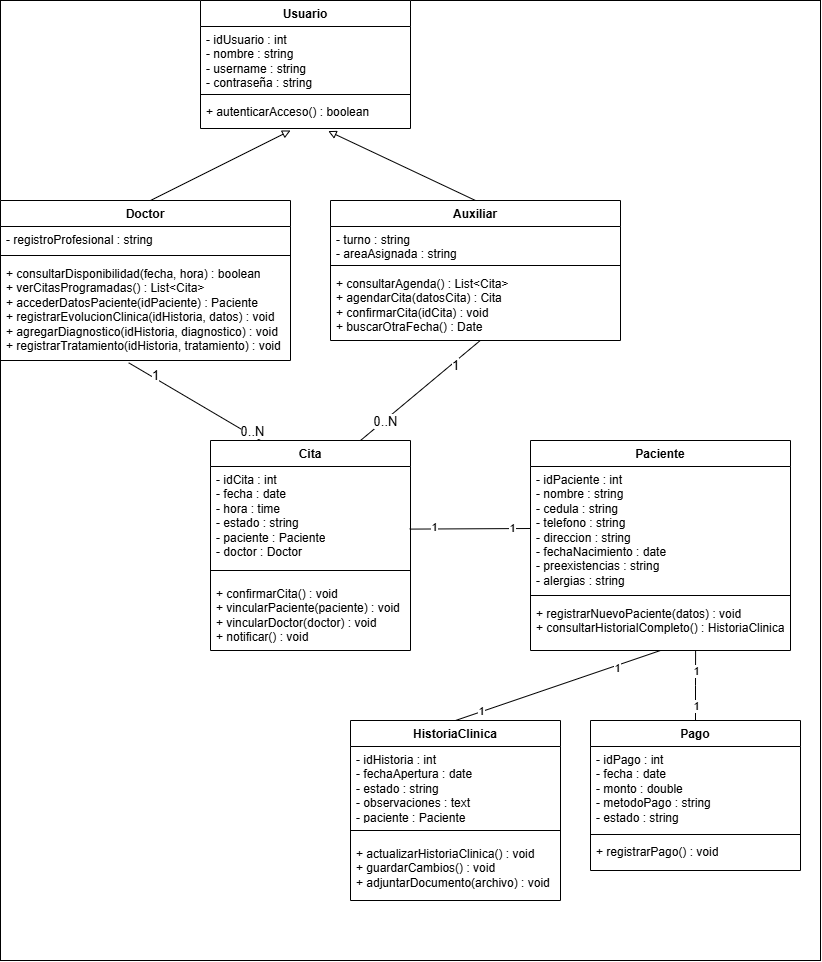
\includegraphics[width=0.5\textwidth]{figuras/diagrama_clases.png}
    \caption{diagrama de clases de la base de datos}. 
 \end{figure}

 \begin{figure}[h!]
     \centering
     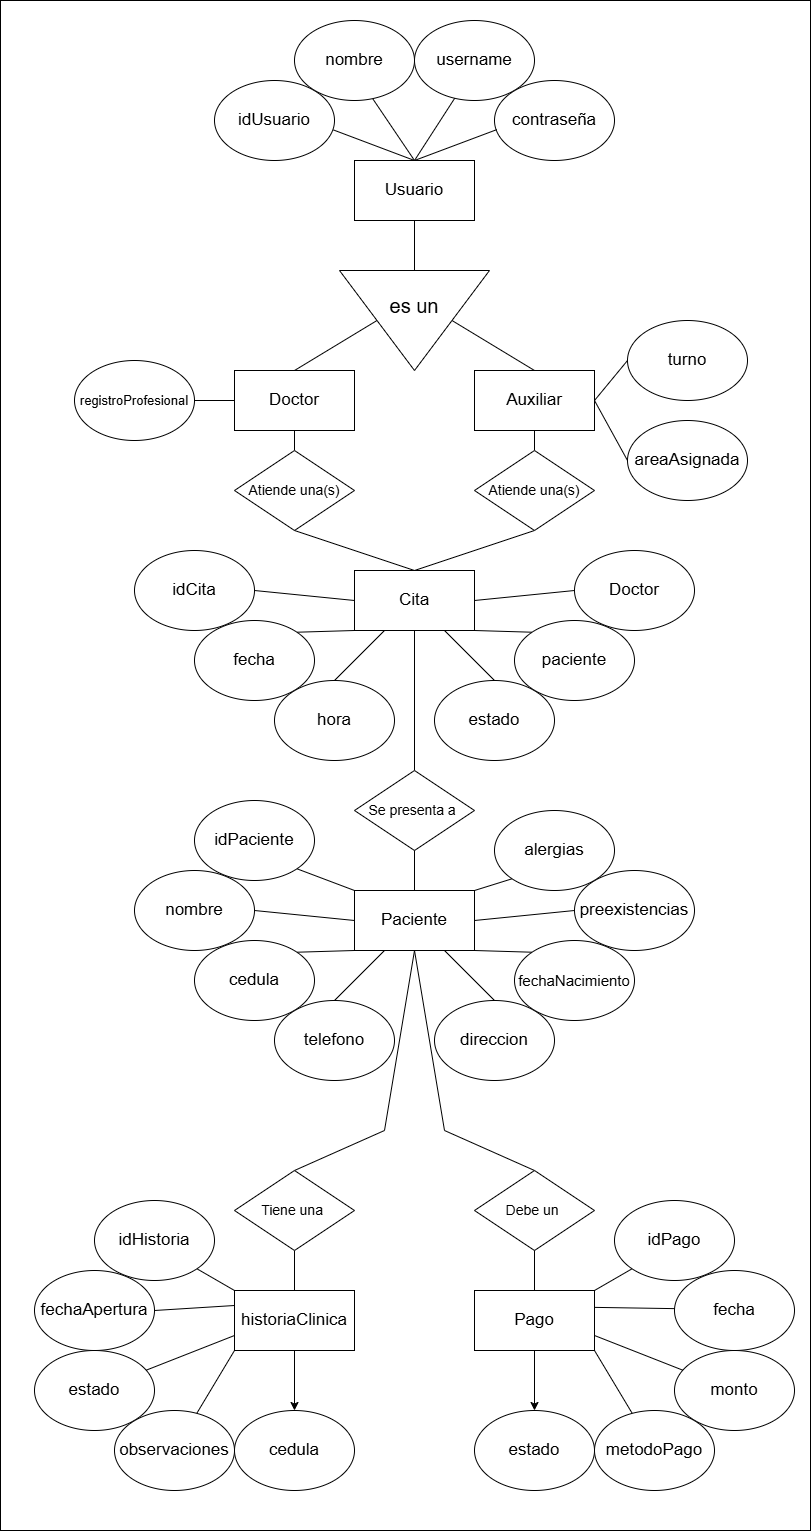
\includegraphics[width=0.5\textwidth]{figuras/MER_actualizado.png}
    \caption{modelo entidad relación de clases de la base de datos}. 
 \end{figure}

\end{document}
